% =====================================================================
%  Introduction to Deep Learning — Class 5
%  Topic (course plan): Single-layer NN/Shallow NN
%  Subtopics (course plan): Regression and Classification
%  This class: the regression half.  Classification follows in Class 6.
%
%  Figures: generated by src/build_all.py (one module per figure).
%  Notation: fixed course convention, Bishop & Bishop (2024) based —
%    x inputs (D of them), y targets, yhat predictions, w weights,
%    phi_j RESERVED for fixed basis functions, a_j pre-activations,
%    z_j = h(a_j) hidden units (M of them), K outputs, N examples.
%
%  Compile:  xelatex main.tex   (run twice)
% =====================================================================

\documentclass[aspectratio=169, 11pt]{beamer}

\usetheme{metropoliscustom}

\usepackage{graphicx}
\DeclareGraphicsExtensions{.pdf,.png,.jpg}
\graphicspath{{figs/}{Class05_Shallow_NN_Regression/B_Recreated_Figures/figs/}}
\usepackage{amsmath, amssymb}
\usepackage{bm}
\usepackage{tikz}
\usetikzlibrary{arrows.meta, positioning, calc, decorations.pathreplacing}
\tcbuselibrary{skins}

\definecolor{mlc}{HTML}{341651}    % ML side (indigo)
\definecolor{nnc}{HTML}{800000}    % NN side (maroon)
\definecolor{tealc}{HTML}{1C7293}  % activations
\definecolor{shc}{HTML}{341651}
\definecolor{dpc}{HTML}{800000}
\definecolor{accc}{HTML}{B8860B}

% ---- theorem environments -------------------------------------------
\setbeamertemplate{theorems}[numbered]
\newtheorem{lemmax}[theorem]{Lemma}
\newtheorem{propx}[theorem]{Proposition}

% ---- parallel-teaching strip: split box, ML left / NN right ----------
%      Compact by design: it always sits above the footer, never in it.
\newcommand{\mlparallel}[2]{%
  \vfill
  {\scriptsize
  \begin{tcolorbox}[enhanced, sidebyside, sidebyside align=top,
                    lefthand ratio=0.485,
                    segmentation style={mlc!35, line width=0.6pt},
                    colback=mlc!5, colframe=mlc!35, boxrule=0.5pt,
                    arc=1.2mm, left=1.6mm, right=1.6mm,
                    top=0.6mm, bottom=0.6mm,
                    before skip=0pt, after skip=0pt]
    {\color{mlc}\textbf{ML}}\hspace{0.55em}#1
  \tcblower
    {\color{nnc}\textbf{NN}}\hspace{0.55em}#2
  \end{tcolorbox}}%
  \vspace{0.35em}%
}

% ---- figure source line (inside a column) ---------------------------
\newcommand{\figsource}[1]{{\scriptsize\color{mcMuted} #1}}

% ---- centred caption under a full-width figure ----------------------
\newcommand{\figcap}[2][0.90]{%
  \begin{center}\begin{minipage}{#1\textwidth}\centering
    {\scriptsize\color{mcMuted} #2}
  \end{minipage}\end{center}}

% ---- a unit drawn as a circle with its activation inside ------------
\newcommand{\unit}[4]{%
  \node[circle, draw=#3, fill=#3!6, line width=1.0pt,
        minimum size=16mm, inner sep=0pt] (#1) at #2 {};
  \begin{scope}
    \clip #2 circle (0.8);
    \draw[tealc, line width=1.6pt]
      ($#2+(-0.80,-0.42)$) -- ($#2+(0.03,-0.42)$) -- ($#2+(0.74,0.45)$);
  \end{scope}
  \node[font=\large, #3] at ($#2+(0,1.12)$) {#4};
}
\newcommand{\plainunit}[4]{%
  \node[circle, draw=#3, fill=black!4, line width=1.0pt,
        minimum size=16mm, inner sep=0pt, font=\normalsize]
        (#1) at #2 {#4};
}

% =====================================================================
\title{Single-layer NN/Shallow NN}
\subtitle{Regression and Classification}
\author{Introduction to Deep Learning \ \textperiodcentered\ Class 5
        \ \textperiodcentered\ Regression}
\institute{}
\date{}

\footleft{Introduction to Deep Learning}
\footright{Single-layer NN/Shallow NN}
\titlelogos{}

\begin{document}

\maketitle

\begin{frame}{Outline}
  \tableofcontents
\end{frame}

% =====================================================================
\section{Regression with Fixed Features}
% =====================================================================

\begin{frame}{Notation used throughout this course}
  \vspace{0.2em}
  {\footnotesize
  \renewcommand{\arraystretch}{1.22}
  \begin{columns}[T, onlytextwidth]
    \begin{column}{0.49\textwidth}
      \begin{tabular}{@{}l@{\hspace{1.6em}}l@{}}
        $\mathbf{x}\in\mathbb{R}^{D}$ & input / \alert{features}\\
        $y$, $\mathbf{y}$ & \alert{target}, targets\\
        $\hat y(\mathbf{x},\mathbf{w})$ & model \alert{prediction}\\
        $N$ & number of examples\\
        $D$, $M$, $K$ & inputs, hidden units, outputs\\
        $\mathbf{w}$, $w_0$ & weights, bias\\
      \end{tabular}
    \end{column}
    \begin{column}{0.49\textwidth}
      \begin{tabular}{@{}l@{\hspace{1.6em}}l@{}}
        $\phi_j(\mathbf{x})$ & \alert{fixed} basis function\\
        $\boldsymbol{\Phi}$ & design matrix, $\Phi_{nj}\!=\!\phi_j(\mathbf{x}_n)$\\
        $a_j$ & pre-activation\\
        $h(\cdot)$ & activation function\\
        $z_j=h(a_j)$ & hidden unit\\
        $E(\mathbf{w})$ & error function\\
      \end{tabular}
    \end{column}
  \end{columns}}
  \vfill
  \begin{redhighlight}
    {\footnotesize Symbols follow \textbf{Bishop \& Bishop (2024)},
    except that targets are written $y$ and predictions $\hat y$.}
  \end{redhighlight}
\end{frame}

\begin{frame}{Linear regression, two views}
  \begin{columns}[T, onlytextwidth]
    \begin{column}{0.44\textwidth}
      \centering
      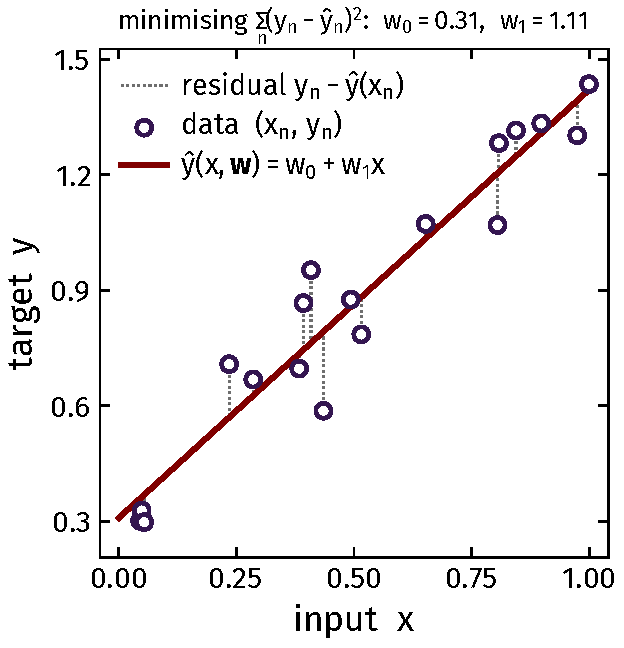
\includegraphics[height=0.40\textheight]{linear_fit}
      \\[0.1em]
      \figsource{$N=18$ noisy points; dotted segments are the
      residuals that get squared and summed.}
    \end{column}
    \hfill
    \begin{column}{0.52\textwidth}
      \vspace{0.3em}
      \[
        \hat y(x,\mathbf{w}) = w_0 + w_1 x
      \]
      \vspace{-0.7em}
      \begin{itemize}\setlength{\itemsep}{0pt}
        \item {\small Two parameters: intercept $w_0$, slope $w_1$}
        \item {\small Fit by minimising the \alert{sum-of-squares
              error}}
        \item {\small A \alert{family} of lines; $\mathbf{w}$ selects
              one member}
      \end{itemize}
    \end{column}
  \end{columns}
  \mlparallel{model $=$ family of functions}
             {parameters select one member --- this framing carries
              through the whole course}
\end{frame}

\begin{frame}{Training: minimise the error}
  \begin{columns}[T, onlytextwidth]
    \begin{column}{0.54\textwidth}
      \centering
      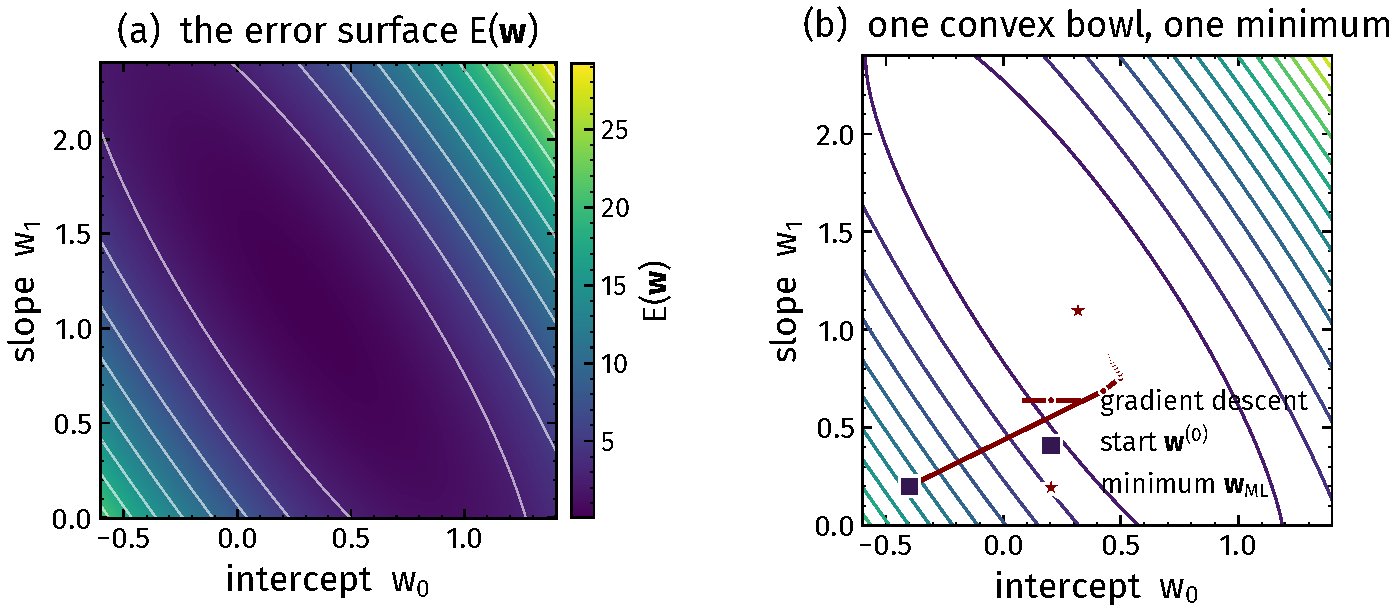
\includegraphics[height=0.44\textheight]{loss_surface}
      \\[0.1em]
      \figsource{(a) the error surface over the two parameters.
      (b) its contours, with gradient descent from a deliberately poor
      start to $\mathbf{w}_{\mathrm{ML}}$.}
    \end{column}
    \hfill
    \begin{column}{0.42\textwidth}
      \vspace{0.3em}
      \[
        E(\mathbf{w})=\tfrac12\sum_{n=1}^{N}
        \big(\hat y(x_n,\mathbf{w})-y_n\big)^2
      \]
      \begin{itemize}\setlength{\itemsep}{2pt}
        \item {\small Each point of $(w_0,w_1)$ space is one
              candidate line}
        \item {\small Walk downhill: \alert{gradient descent}}
        \item {\small For a model \alert{linear in} $\mathbf{w}$ this
              surface is convex --- one minimum, and a closed form}
      \end{itemize}
    \end{column}
  \end{columns}
\end{frame}

\begin{frame}{Beyond lines: fixed basis functions}
  \[
    \hat y(\mathbf{x},\mathbf{w})
    = \sum_{j=0}^{M-1} w_j\,\phi_j(\mathbf{x})
    = \mathbf{w}^{\!\top}\boldsymbol{\phi}(\mathbf{x})
    \tag{B\&B 4.3}
  \]
  \vspace{-0.7em}
  \begin{center}
    {\small Chosen \alert{before} seeing data; only $\mathbf{w}$ is
    learned --- still \alert{linear in} $\mathbf{w}$, nonlinear in
    $\mathbf{x}$.}
  \end{center}
  \vspace{-0.5em}
  \begin{center}
    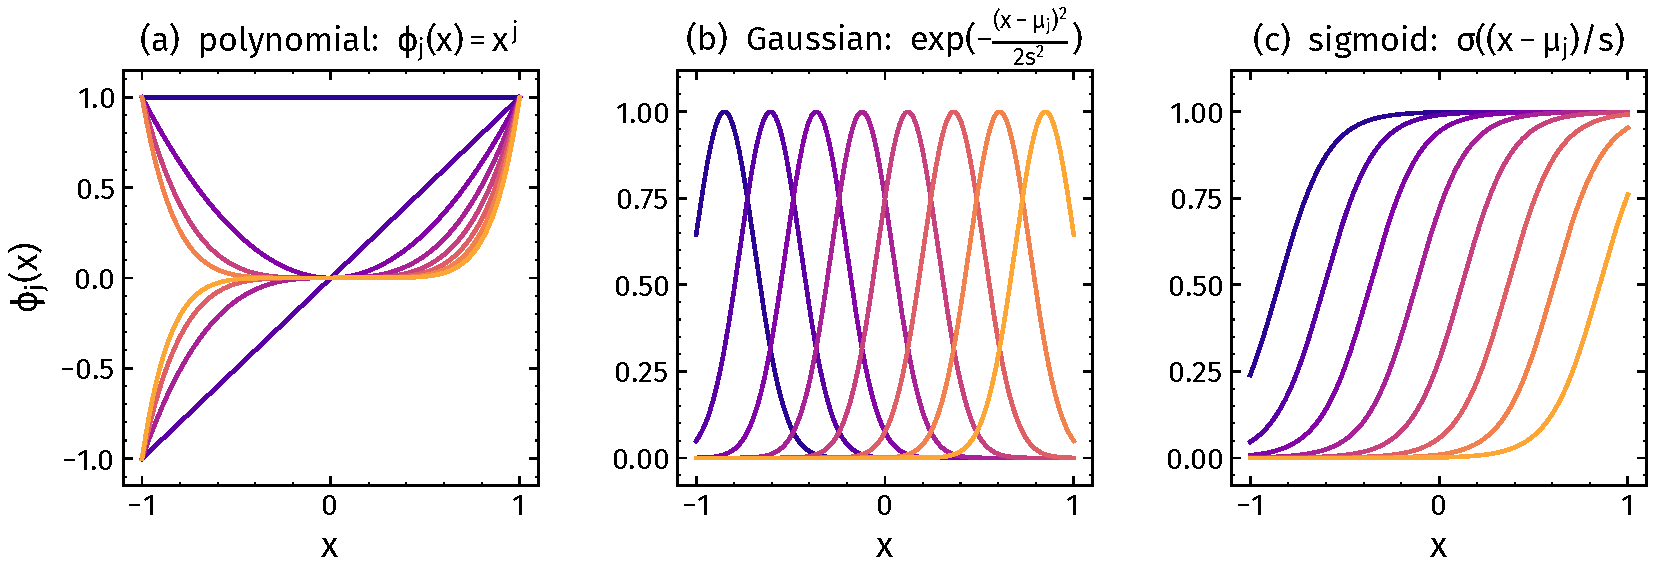
\includegraphics[height=0.28\textheight]{basis_functions}
  \end{center}
  \vspace{-0.2em}
  \figcap[0.96]{Three classical families, eight members each.}
\end{frame}

\begin{frame}{Result: the normal equations}
  \begin{theorem}[Least-squares solution]
    Let $\boldsymbol{\Phi}\in\mathbb{R}^{N\times M}$ have
    $\Phi_{nj}=\phi_j(\mathbf{x}_n)$ and let
    $E(\mathbf{w})=\tfrac12\lVert\boldsymbol{\Phi}\mathbf{w}
    -\mathbf{y}\rVert^2$.
    If $\boldsymbol{\Phi}$ has full column rank, $E$ has the unique
    minimiser
    \[
      \mathbf{w}_{\mathrm{ML}}
      = \big(\boldsymbol{\Phi}^{\!\top}\boldsymbol{\Phi}\big)^{-1}
        \boldsymbol{\Phi}^{\!\top}\mathbf{y}
      \;=\;\boldsymbol{\Phi}^{\dagger}\mathbf{y}.
      \tag{B\&B 4.14}
    \]
  \end{theorem}
  \vspace{0.2em}
  {\footnotesize
  \begin{itemize}\setlength{\itemsep}{1pt}
    \item \focus{1}{$\nabla_{\mathbf{w}}E
          = \boldsymbol{\Phi}^{\!\top}
          (\boldsymbol{\Phi}\mathbf{w}-\mathbf{y})$ \quad
          (differentiate the quadratic)}
    \item \focus{2}{Set it to $\mathbf{0}$:
          $\;\boldsymbol{\Phi}^{\!\top}\boldsymbol{\Phi}\,\mathbf{w}
          =\boldsymbol{\Phi}^{\!\top}\mathbf{y}$ \quad
          --- the \alert{normal equations}}
    \item \focus{3}{$\nabla^2_{\mathbf{w}}E
          =\boldsymbol{\Phi}^{\!\top}\boldsymbol{\Phi}\succ 0$ under
          full rank, so the stationary point is the global minimum}
    \item \focus{4}{Invert:
          $\mathbf{w}_{\mathrm{ML}}
          =(\boldsymbol{\Phi}^{\!\top}\boldsymbol{\Phi})^{-1}
          \boldsymbol{\Phi}^{\!\top}\mathbf{y}$
          \hfill $\square$}
  \end{itemize}}
\end{frame}

\begin{frame}{Least squares in closed form: the geometry}
  \begin{columns}[T, onlytextwidth]
    \begin{column}{0.54\textwidth}
      \vspace{0.2em}
      \begin{propx}[Orthogonal projection]
        {\footnotesize $\hat{\mathbf{y}}
        =\boldsymbol{\Phi}\mathbf{w}_{\mathrm{ML}}$ is the orthogonal
        projection of $\mathbf{y}$ onto
        $\mathcal{S}=\mathrm{span}\{\bm\varphi_1,\dots,\bm\varphi_M\}$.}
      \end{propx}
      {\footnotesize
      \emph{Proof.} The normal equations read
      $\boldsymbol{\Phi}^{\!\top}(\mathbf{y}-\hat{\mathbf{y}})
      =\mathbf{0}$, i.e.\ the residual is orthogonal to every column
      $\bm\varphi_j$, hence to all of $\mathcal{S}$. \hfill$\square$}
      \vspace{0.3em}
      {\footnotesize
      \begin{itemize}\setlength{\itemsep}{0pt}
        \item Columns $\bm\varphi_j\in\mathbb{R}^N$ span an
              $M$-dimensional subspace of $\mathbb{R}^N$
        \item Least squares $=$ \alert{drop a perpendicular}
      \end{itemize}}
    \end{column}
    \hfill
    \begin{column}{0.42\textwidth}
      \centering
      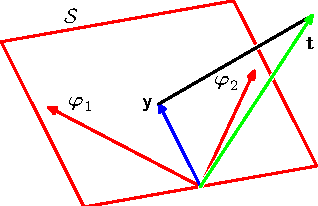
\includegraphics[height=0.40\textheight]{Bishop4_3}
      \\[0.1em]
      \figsource{Figure from Bishop \& Bishop (2024), Fig.~4.3.
      $\mathbf{t}$ there is our target vector $\mathbf{y}$.}
    \end{column}
  \end{columns}
  \mlparallel{closed form exists}
             {parameters inside $h(\cdot)$ destroy it}
\end{frame}

\begin{frame}{Why least squares? The probabilistic view}
  \begin{columns}[T, onlytextwidth]
    \begin{column}{0.50\textwidth}
      \vspace{0.2em}
      \begin{propx}[Least squares $=$ maximum likelihood]
        {\footnotesize Under
        $p(y\mid\mathbf{x},\mathbf{w},\sigma^2)
        =\mathcal{N}\big(y\mid\hat y(\mathbf{x},\mathbf{w}),
        \sigma^2\big)$ with i.i.d.\ data, maximising the likelihood
        in $\mathbf{w}$ is equivalent to minimising
        $\sum_n(y_n-\hat y_n)^2$.}
      \end{propx}
      {\footnotesize
      \emph{Proof.}
      $\ln p(\mathbf{y}\mid\mathbf{w},\sigma^2)
      = -\frac{1}{2\sigma^2}\sum_n(y_n-\hat y_n)^2
      -\frac{N}{2}\ln\sigma^2-\frac{N}{2}\ln 2\pi$.
      Only the first term involves $\mathbf{w}$, and $\sigma^2>0$,
      so the two problems have the same argmin.
      \hfill$\square$}
    \end{column}
    \hfill
    \begin{column}{0.46\textwidth}
      \centering
      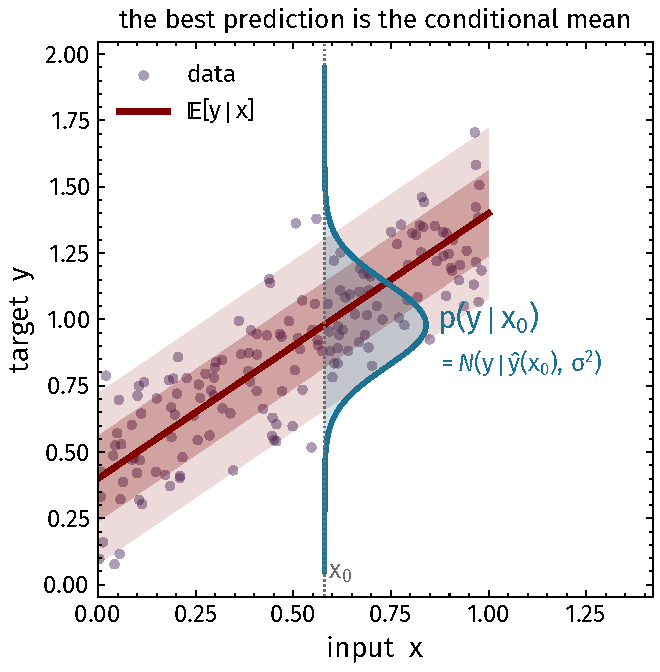
\includegraphics[height=0.335\textheight]{conditional_mean}
      \\[0.1em]
      \figsource{Bands are $\pm1$ and $\pm2$ standard deviations; the
      turquoise curve is $p(y\mid x_0)$ at one input.}
    \end{column}
  \end{columns}
  \vspace{0.8em}
  \mlparallel{Gaussian noise $\to$ squared error}
             {Class 6: Bernoulli noise $\to$ cross-entropy}
\end{frame}

\begin{frame}{What is the best possible prediction?}
  \begin{theorem}[The optimal predictor is the conditional mean]
    {\small For squared loss, the function minimising
    $\mathbb{E}_{\mathbf{x},y}\big[(f(\mathbf{x})-y)^2\big]$ over all
    measurable $f$ is $f^{*}(\mathbf{x})=\mathbb{E}[y\mid\mathbf{x}]$,
    and for any $f$,
    \[
      \mathbb{E}\big[(f-y)^2\big]
      = \underbrace{\int\!\big(f(\mathbf{x})-f^{*}(\mathbf{x})\big)^2
        p(\mathbf{x})\,\mathrm{d}\mathbf{x}}_{\text{what the model
        controls}}
      +
      \underbrace{\int\!\mathrm{var}\,[y\mid\mathbf{x}]\,
        p(\mathbf{x})\,\mathrm{d}\mathbf{x}}_{\text{intrinsic noise}}.
    \]}
  \end{theorem}
  \vspace{-0.3em}
  {\scriptsize
  \emph{Proof.} Write $f-y=(f-f^{*})+(f^{*}-y)$ and expand. The cross
  term vanishes because
  $\mathbb{E}[f^{*}(\mathbf{x})-y\mid\mathbf{x}]=0$ by definition of
  $f^{*}$; both remaining terms are non-negative and the second is
  free of $f$. \hfill$\square$ \;{\itshape B\&B, 2024, \S4.2}}
  \vspace{-0.3em}
  \begin{redhighlight}
    {\scriptsize The noise floor is \alert{irreducible}. All a network
    can do is close the first term --- which is exactly why we care how
    rich its function family is.}
  \end{redhighlight}
\end{frame}

\begin{frame}{Linear regression is itself a network}
  \begin{columns}[T, onlytextwidth]
    \begin{column}{0.42\textwidth}
      \centering
      \begin{tikzpicture}[>=Stealth, line width=0.8pt,
      scale=0.50, transform shape, font=\normalsize]
    \foreach \i/\y in {0/2.4, 1/0.8, {M-1}/-2.4}{
      \node[circle, draw=shc, fill=shc!8, line width=1.0pt,
            minimum size=13mm, inner sep=0pt] (p\i) at (0,\y)
            {$\phi_{\i}$};
      \draw[->, black!55] (p\i) -- node[above, pos=0.55, font=\small,
        black!70] {$w_{\i}$} (3.2,0.0);
    }
    \node at (0,-0.9) {$\vdots$};
    \node[circle, draw=dpc, fill=dpc!6, line width=1.2pt,
          minimum size=15mm, inner sep=0pt] (o) at (3.9,0.0)
          {\large$\displaystyle\sum$};
    \draw[->, black!55] (o) -- (5.9,0.0);
    \node[right, font=\normalsize] at (5.95,0.0) {$\hat y$};
    \node[font=\small, shc] at (0,3.35) {basis functions};
  \end{tikzpicture}
      \\[0.1em]
      \figsource{One node per basis function, one weight per link,
      summed at the output.}
    \end{column}
    \hfill
    \begin{column}{0.54\textwidth}
      \vspace{0.2em}
      {\footnotesize
      \begin{itemize}\setlength{\itemsep}{0pt}
        \item Nodes: $\phi_j(\mathbf{x})$; links: weights $w_j$
        \item Already a one-layer network --- but the $\phi_j$
              \alert{carry no parameters}
      \end{itemize}}
      \vspace{0.2em}
      \begin{alertblock}{The limitation}
        {\footnotesize For images, audio and text nobody knows how to
        write good $\phi_j$ by hand.}
      \end{alertblock}
    \end{column}
  \end{columns}
  \mlparallel{$\phi_j$ fixed by design}
             {next: give the basis functions \emph{parameters}}
\end{frame}

\begin{frame}{Why shallow networks}
  A linear model in fixed features is limited. We want a model that
  is:
  \vspace{0.3em}
  \begin{itemize}
    \item flexible enough to describe \alert{arbitrarily complex}
          input--output mappings,
    \item able to take \alert{as many inputs} as we want,
    \item able to produce \alert{as many outputs} as we want.
  \end{itemize}
  \vspace{0.5em}
  \begin{redhighlight}
    Shallow neural networks do all three --- by putting parameters
    \emph{inside} the basis functions and learning them from data.
  \end{redhighlight}
\end{frame}

% =====================================================================
\section{An Example Shallow Network}
% =====================================================================

\begin{frame}{The model}
  Scalar input $x$, scalar output, $M=3$ hidden units, ten
  parameters (Bishop \& Bishop, 2024, Eqs.~6.1--6.3):
  \[
    a_j = w^{(1)}_{j0} + w^{(1)}_{j1}x, \qquad
    z_j = h(a_j), \qquad
    \hat y = w^{(2)}_{0} + \sum_{j=1}^{M} w^{(2)}_{j} z_j
  \]
  \vspace{-0.3em}
  \begin{itemize}\setlength{\itemsep}{1pt}
    \item {\small Compare $\hat y=\sum_j w_j\phi_j(\mathbf{x})$:
          the same outer form, but the features $z_j$ now
          \alert{contain parameters}}
    \item {\small Given $\mathbf{w}$: inference $=$ evaluate the
          three equations}
    \item {\small Given data: same sum-of-squares $E(\mathbf{w})$,
          minimised over \emph{all} the weights}
  \end{itemize}
  \mlparallel{$\mathbf{w}^{\!\top}\boldsymbol{\phi}(\mathbf{x})$:
              linear in \emph{fixed} features}
             {$\sum_j w^{(2)}_j z_j$: linear in
              \emph{parameterised} features}
\end{frame}

\begin{frame}{The activation function: ReLU}
  \begin{columns}[T, onlytextwidth]
    \begin{column}{0.46\textwidth}
      \vspace{0.9em}
      \[
        h(a)=\mathrm{ReLU}(a)=\max(0,a)=
        \begin{cases} 0 & a<0\\ a & a\ge 0\end{cases}
      \]
      \vspace{0.5em}
      \begin{itemize}\setlength{\itemsep}{5pt}
        \item {\small The \alert{rectified linear unit}: clips
              negative pre-activations to zero}
        \item {\small Without it the model collapses:
              $\sum_j w^{(2)}_j(w^{(1)}_{j0}+w^{(1)}_{j1}x)$ is
              just a line again}
      \end{itemize}
    \end{column}
    \hfill
    \begin{column}{0.48\textwidth}
      \centering
      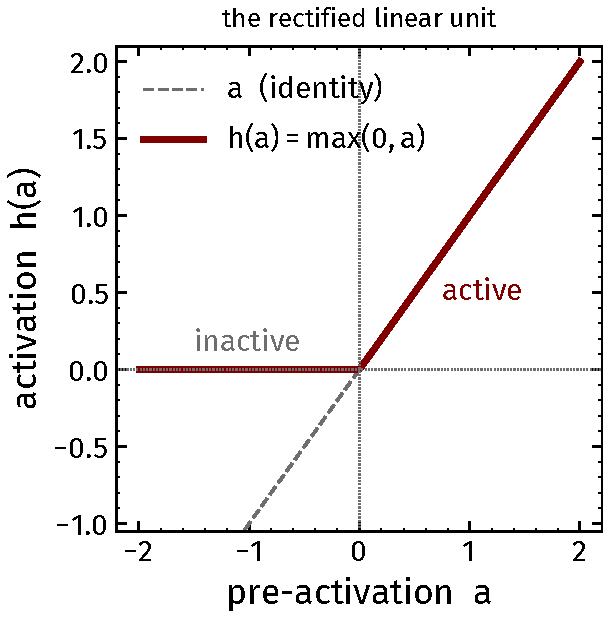
\includegraphics[height=0.475\textheight]{relu}
      \\[0.2em]
      \figsource{Positive pre-activations pass through unchanged;
      everything negative is clipped to zero.}
    \end{column}
  \end{columns}
  \mlparallel{fixed nonlinearity: $x^j$, Gaussian, sigmoid}
             {nonlinearity applied to a \emph{learned} line}
\end{frame}

\begin{frame}{Hidden units: the model in two stages}
  Stage 1 --- three linear functions, each passed through $h$:
  \[
    z_1=h\big(w^{(1)}_{10}+w^{(1)}_{11}x\big), \quad
    z_2=h\big(w^{(1)}_{20}+w^{(1)}_{21}x\big), \quad
    z_3=h\big(w^{(1)}_{30}+w^{(1)}_{31}x\big)
  \]
  \vfill
  Stage 2 --- weight and sum:
  \[
    \hat y = w^{(2)}_0+w^{(2)}_1 z_1+w^{(2)}_2 z_2+w^{(2)}_3 z_3
  \]
  \vfill
  \begin{itemize}\setlength{\itemsep}{4pt}
    \item {\small $z_1,z_2,z_3$ are the \alert{hidden units}}
    \item {\small Clipped $\to$ \alert{inactive}; passing its input
          $\to$ \alert{active}}
  \end{itemize}
  \mlparallel{regress $y$ on fixed $\boldsymbol{\phi}(\mathbf{x})$}
             {Stage~2 \emph{is} that regression, on learned $z$}
\end{frame}

\begin{frame}{Computing the function, step by step}
  \begin{center}
    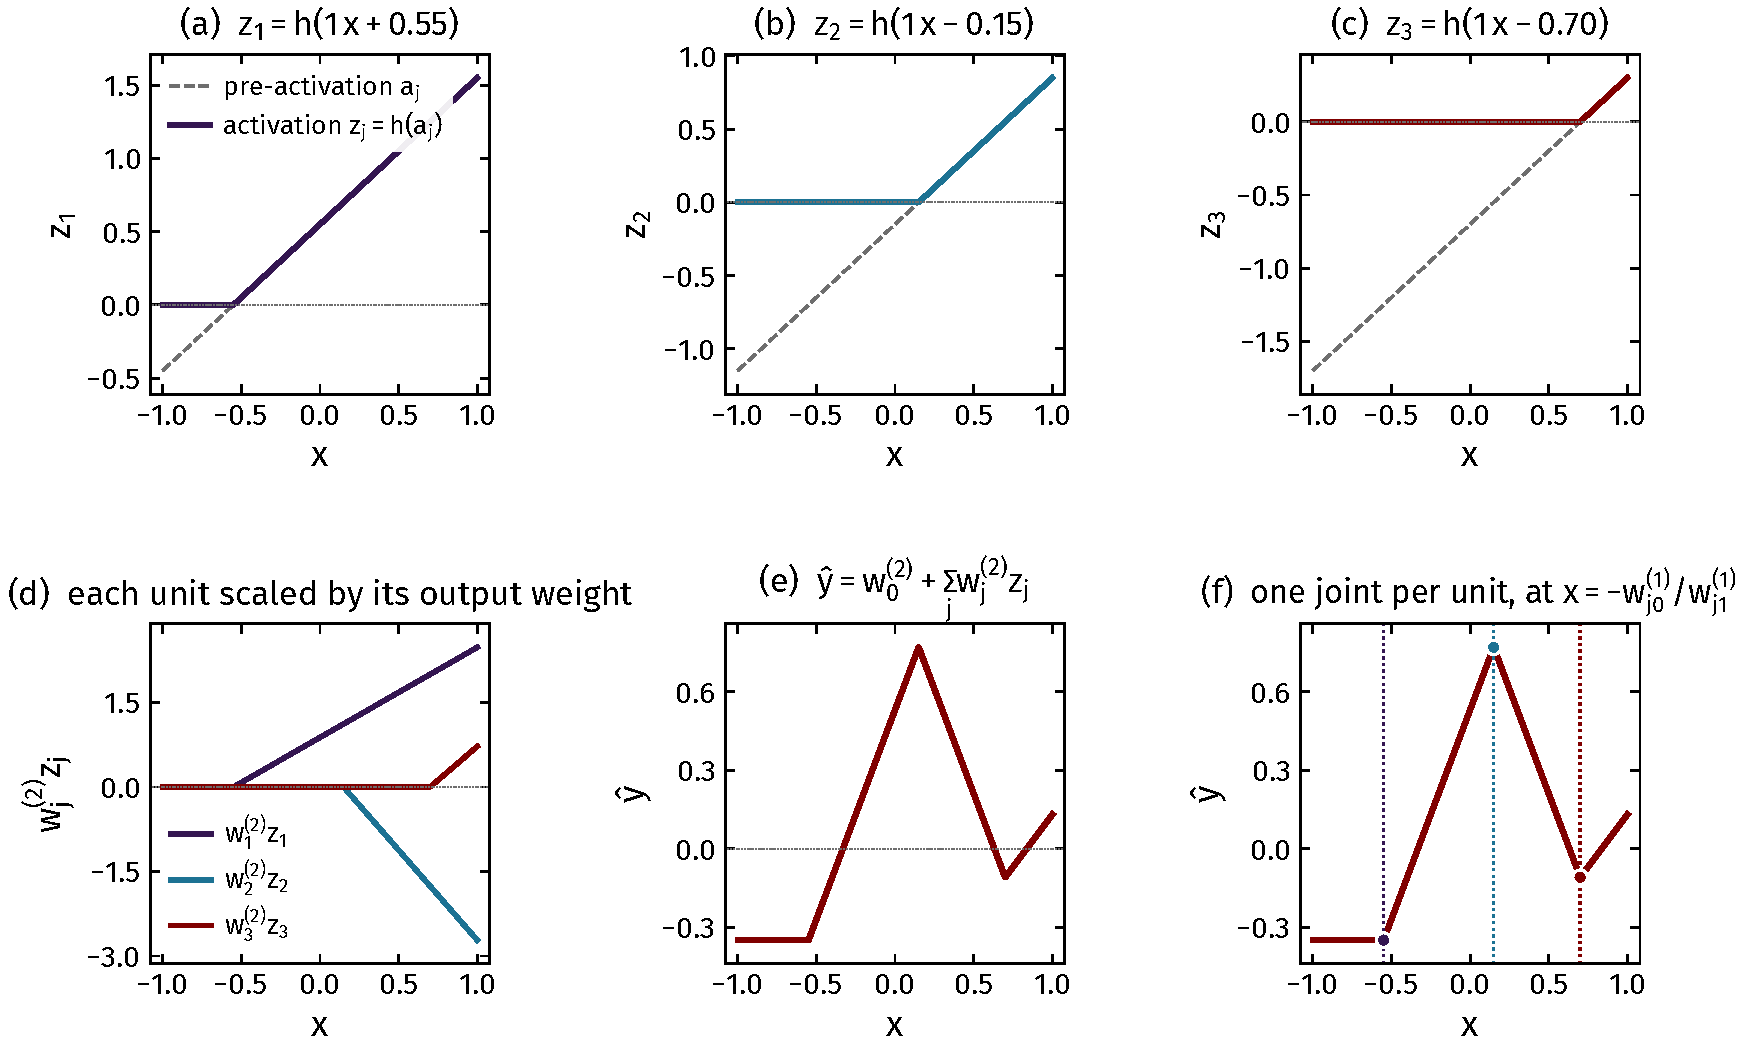
\includegraphics[height=0.605\textheight]{buildup}
  \end{center}
  \vspace{-0.2em}
  \vspace{-0.1em}
  \figcap[0.98]{(a--c) one unit each: dashed $a_j$, solid $z_j=h(a_j)$.
  (d) scaled by $w^{(2)}_j$. (e) summed, plus $w^{(2)}_0$.
  (f) the joints.}
\end{frame}

\begin{frame}{The function family: piecewise linear}
  \begin{columns}[T, onlytextwidth]
    \begin{column}{0.60\textwidth}
      \centering
      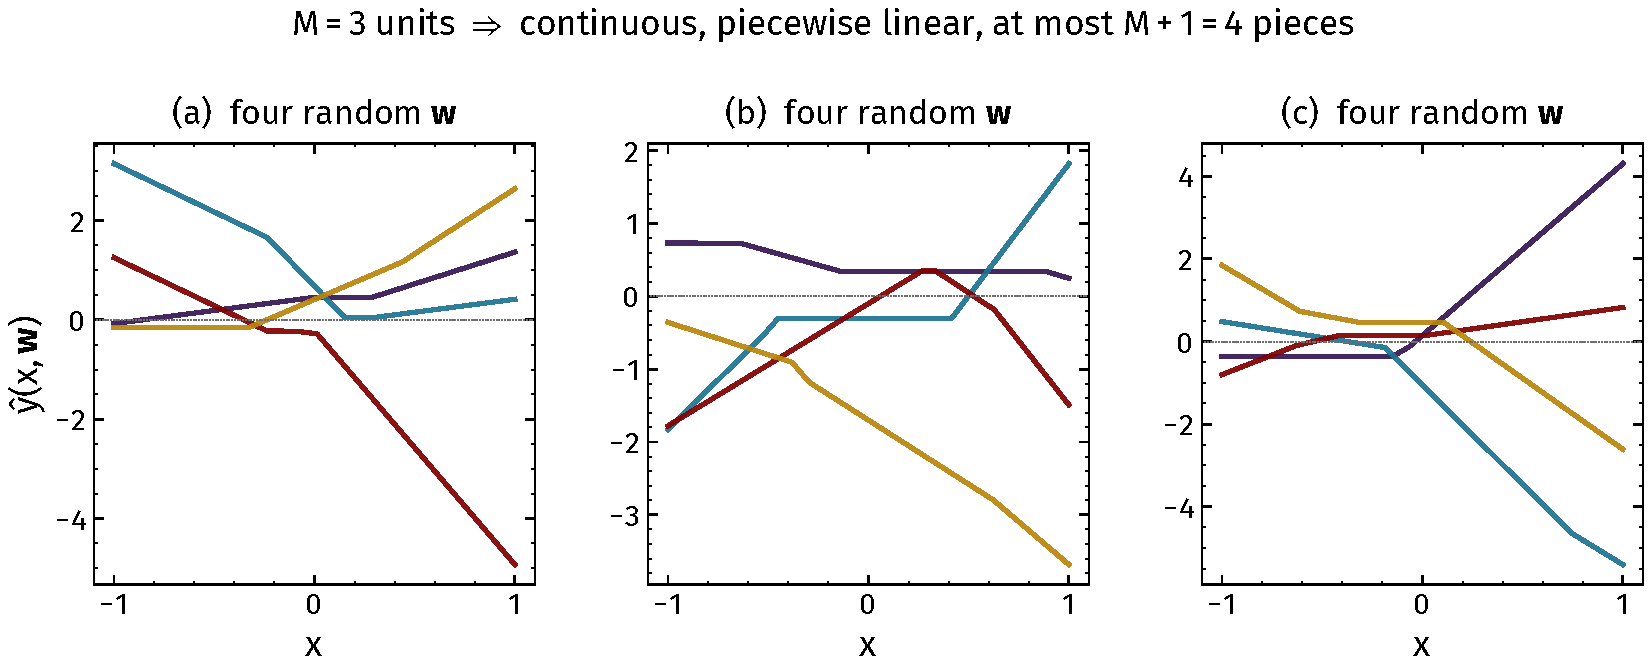
\includegraphics[width=\linewidth]{family}
      \\[0.2em]
      \figsource{Twelve networks with $M=3$ units and randomly drawn
      weights: all continuous and piecewise linear, differing only in
      where the joints fall and how steep each piece is.}
    \end{column}
    \hfill
    \begin{column}{0.36\textwidth}
      \vspace{0.3em}
      {\small
      \begin{itemize}\setlength{\itemsep}{2pt}
        \item Continuous piecewise-linear functions
        \item One \alert{joint per ReLU}, at
              $x=-w^{(1)}_{j0}/w^{(1)}_{j1}$
        \item Each region $\leftrightarrow$ an \alert{activation
              pattern}: which units are on
      \end{itemize}}
    \end{column}
  \end{columns}
  \mlparallel{family: span of the chosen $\phi_j$}
             {family: piecewise linear, joints placed by training}
\end{frame}

\begin{frame}{Depicting the network}
  \centering
  \begin{tikzpicture}[>=Stealth, line width=0.8pt,
      scale=0.48, transform shape, font=\normalsize]
    \plainunit{i}{(0,0)}{black!55}{$x$}
    \unit{a1}{(2.6,2.3)}{shc}{$z_1$}
    \unit{a2}{(2.6,0.0)}{shc}{$z_2$}
    \unit{a3}{(2.6,-2.3)}{shc}{$z_3$}
    \plainunit{o}{(5.2,0)}{dpc}{$\hat y$}
    \foreach \i in {1,2,3} \draw[->, black!45]
      (i)-- node[above, pos=0.6, font=\small, black!65]
      {$w^{(1)}_{\i1}$} (a\i);
    \foreach \i in {1,2,3} \draw[->, black!45]
      (a\i)-- node[above, pos=0.4, font=\small, black!65]
      {$w^{(2)}_{\i}$} (o);
    \node[font=\small, shc] at (2.6,3.9) {hidden layer};
  \end{tikzpicture}
  \\[0.2em]
  \figcap[0.86]{Each arrow carries one weight; the turquoise glyph
  inside a unit marks where the activation $h$ is applied. Biases
  $w^{(1)}_{j0}$ and $w^{(2)}_0$ are not drawn.}
  \vspace{0.2em}
  {\small
  \begin{itemize}\setlength{\itemsep}{1pt}
    \item Each \alert{weight multiplies its source and adds to its
          target}
    \item Ten parameters: six into the hidden layer, four out of it
  \end{itemize}}
\end{frame}

\begin{frame}{Hidden units are basis functions that adapt}
  \begin{center}
    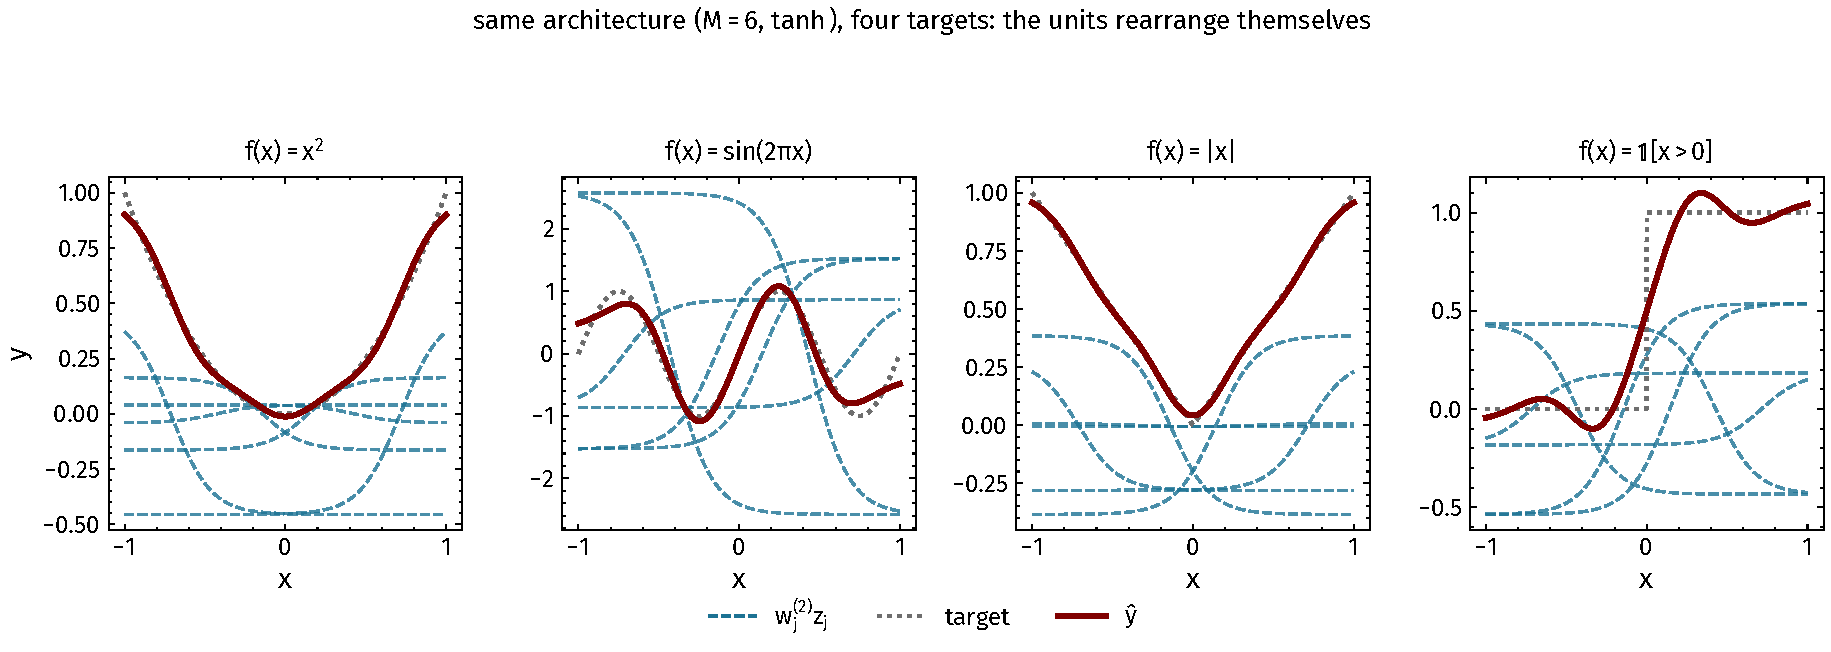
\includegraphics[height=0.335\textheight]{learned_basis}
  \end{center}
  \figcap[0.92]{Dashed: the individual weighted hidden units
  $w^{(2)}_j z_j$ after fitting. Dotted: the target. Solid: the
  network output. The same architecture rearranges its units
  differently for each target.}
  \vspace{0.2em}
  {\small
  \begin{itemize}\setlength{\itemsep}{1pt}
    \item Same $M$, same activation --- but the effective basis is
          \alert{chosen by the data}
    \item This is the whole difference from
          $\hat y=\mathbf{w}^{\!\top}\boldsymbol\phi(\mathbf{x})$
  \end{itemize}}
\end{frame}

% =====================================================================
\section{Generalising the Network}
% =====================================================================

\begin{frame}{Capacity: $M$ hidden units}
  \[
    z_j=h\big(w^{(1)}_{j0}+w^{(1)}_{j1}x\big),
    \qquad
    \hat y=w^{(2)}_0+\sum_{j=1}^{M}w^{(2)}_j z_j
  \]
  \begin{itemize}
    \item The number of hidden units $M$ is a measure of
          \alert{network capacity}
    \item $M$ ReLU units on a scalar input give $M$ joints, hence at
          most \alert{$M{+}1$ linear regions}
    \item Parameter count for $D$ inputs, $M$ units, $K$ outputs:
          $M(D{+}1)+K(M{+}1)$
  \end{itemize}
  \mlparallel{capacity dial: number of basis functions $M$}
             {capacity dial: number of hidden units $M$}
\end{frame}

\begin{frame}{More than one output}
  \begin{columns}[T, onlytextwidth]
    \begin{column}{0.60\textwidth}
      \centering
      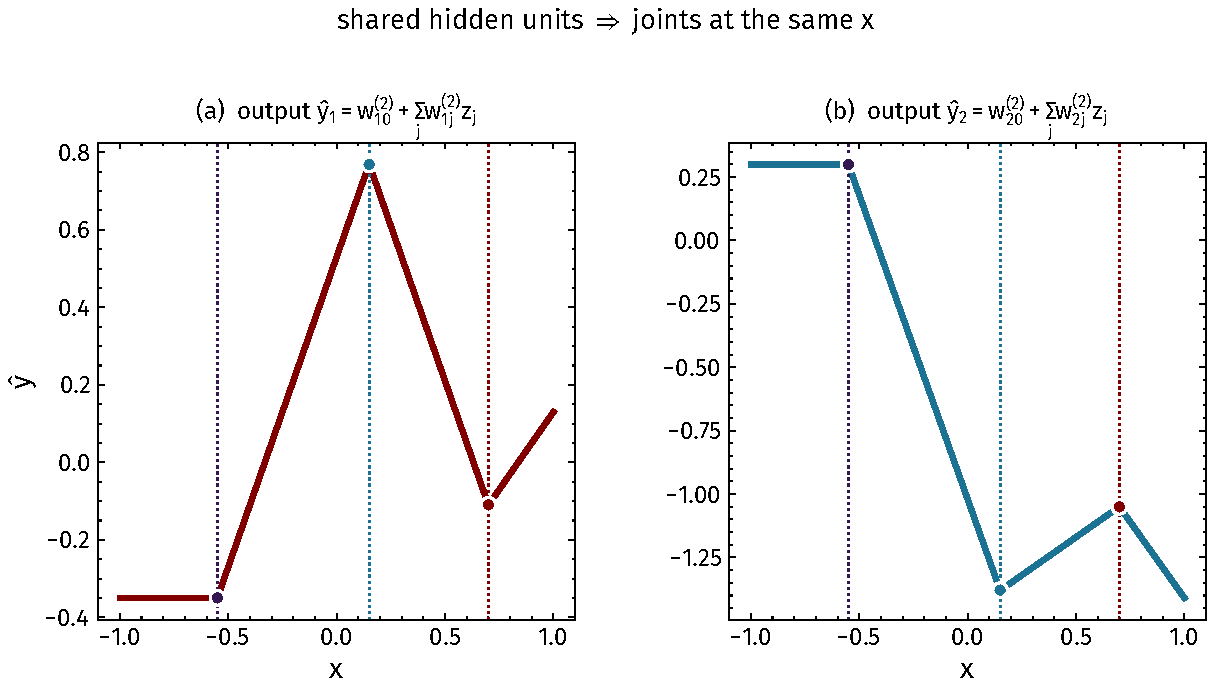
\includegraphics[width=\linewidth]{two_outputs}
      \\[0.2em]
      \figsource{Coloured markers are the joints. Both outputs bend
      at exactly the same $x$, because they read the same $z_j$.}
    \end{column}
    \hfill
    \begin{column}{0.36\textwidth}
      \vspace{0.3em}
      {\small $D=1$, $M=4$, $K=2$:}
      \[
        \hat y_k=w^{(2)}_{k0}+\sum_{j=1}^{M}w^{(2)}_{kj}z_j
      \]
      {\small
      \begin{itemize}\setlength{\itemsep}{2pt}
        \item One extra linear read-out per output; the hidden units
              are \alert{shared}
        \item Hence the joints sit at the \alert{same places}
      \end{itemize}}
    \end{column}
  \end{columns}
\end{frame}

\begin{frame}{More than one input}
  \begin{columns}[T, onlytextwidth]
    \begin{column}{0.46\textwidth}
      \centering
      \begin{tikzpicture}[>=Stealth, line width=0.8pt,
      scale=0.46, transform shape, font=\normalsize]
    \plainunit{i1}{(0,1.3)}{black!55}{$x_1$}
    \plainunit{i2}{(0,-1.3)}{black!55}{$x_2$}
    \unit{h1}{(3.0,2.4)}{shc}{$z_1$}
    \unit{h2}{(3.0,0.0)}{shc}{$z_2$}
    \unit{h3}{(3.0,-2.4)}{shc}{$z_3$}
    \plainunit{o}{(6.0,0)}{dpc}{$\hat y$}
    \foreach \i in {1,2} \foreach \j in {1,2,3}
      \draw[->, black!30] (i\i)--(h\j);
    \foreach \j in {1,2,3} \draw[->, black!45] (h\j)--(o);
    \node[font=\small] at (0,3.2) {$D=2$ inputs};
    \node[font=\small, shc] at (3.0,4.0) {$M=3$ units};
  \end{tikzpicture}
      \\[0.1em]
      \figsource{Every hidden unit now receives \emph{both} inputs,
      so each has two slopes and one bias.}
    \end{column}
    \hfill
    \begin{column}{0.50\textwidth}
      \vspace{0.4em}
      \[
        a_j=w^{(1)}_{j0}+w^{(1)}_{j1}x_1+w^{(1)}_{j2}x_2,
        \quad z_j=h(a_j)
      \]
      \[
        \hat y=w^{(2)}_0+\sum_{j=1}^{3}w^{(2)}_j z_j
      \]
      \vspace{-0.4em}
      {\footnotesize
      \begin{itemize}\setlength{\itemsep}{2pt}
        \item Each pre-activation is an \alert{oriented plane} over
              the input space
        \item $a_j=0$ is a \alert{line}: on one side the unit is
              off, on the other it rises linearly
      \end{itemize}}
    \end{column}
  \end{columns}
  \vspace{1.1em}
  \mlparallel{$\phi_j:\mathbb{R}^D\to\mathbb{R}$, hand-designed}
             {$z_j:\mathbb{R}^D\to\mathbb{R}$, an oriented hinge,
              learned}
\end{frame}

\begin{frame}{Each unit is a hinge over the input plane}
  \begin{center}
    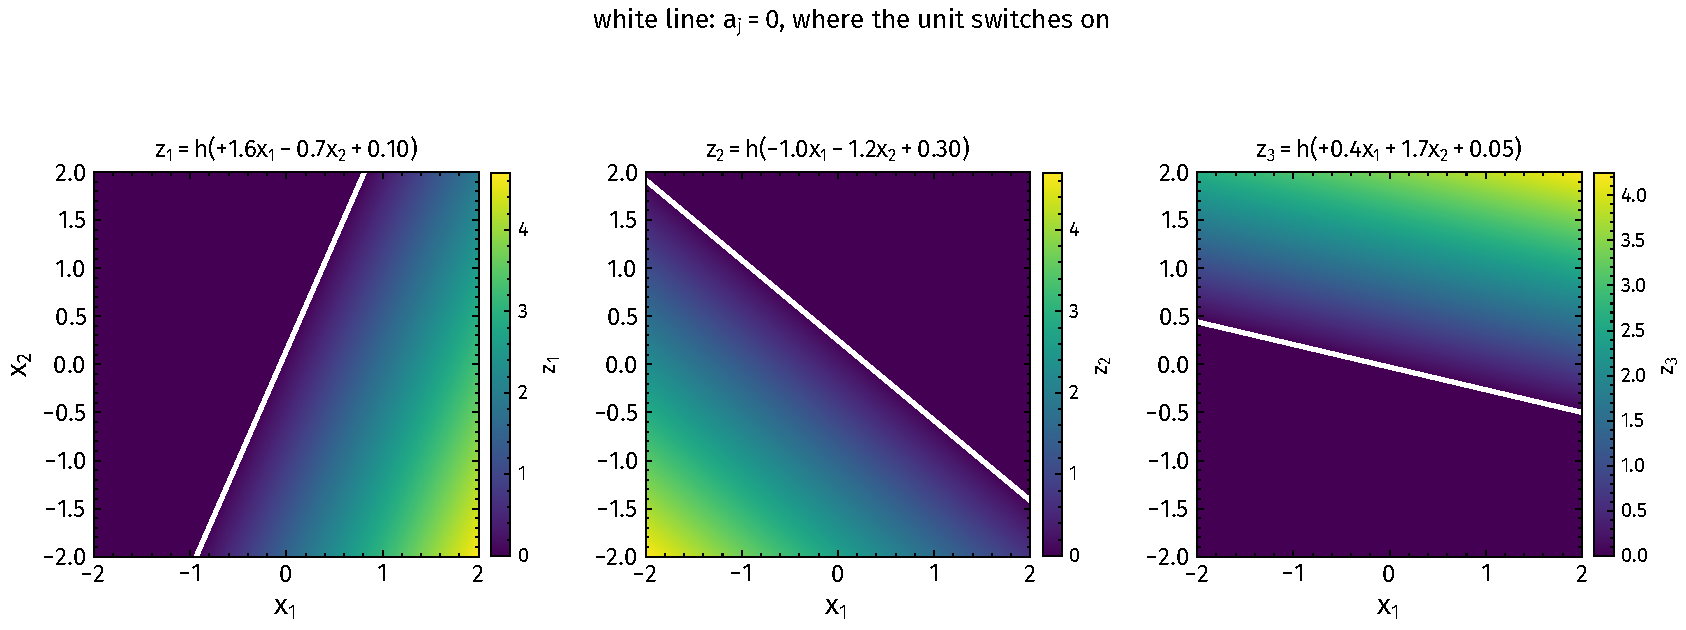
\includegraphics[height=0.55\textheight]{two_inputs}
  \end{center}
  \figcap[0.94]{The three hidden units of that network, drawn over
  $(x_1,x_2)$. Each is flat (dark) on one side of its white line
  $a_j=0$ and rises linearly on the other; the orientation and
  offset of the line are set by $w^{(1)}_{j1},w^{(1)}_{j2}$ and
  $w^{(1)}_{j0}$.}
\end{frame}

\begin{frame}{Two inputs, computed step by step}
  \begin{center}
    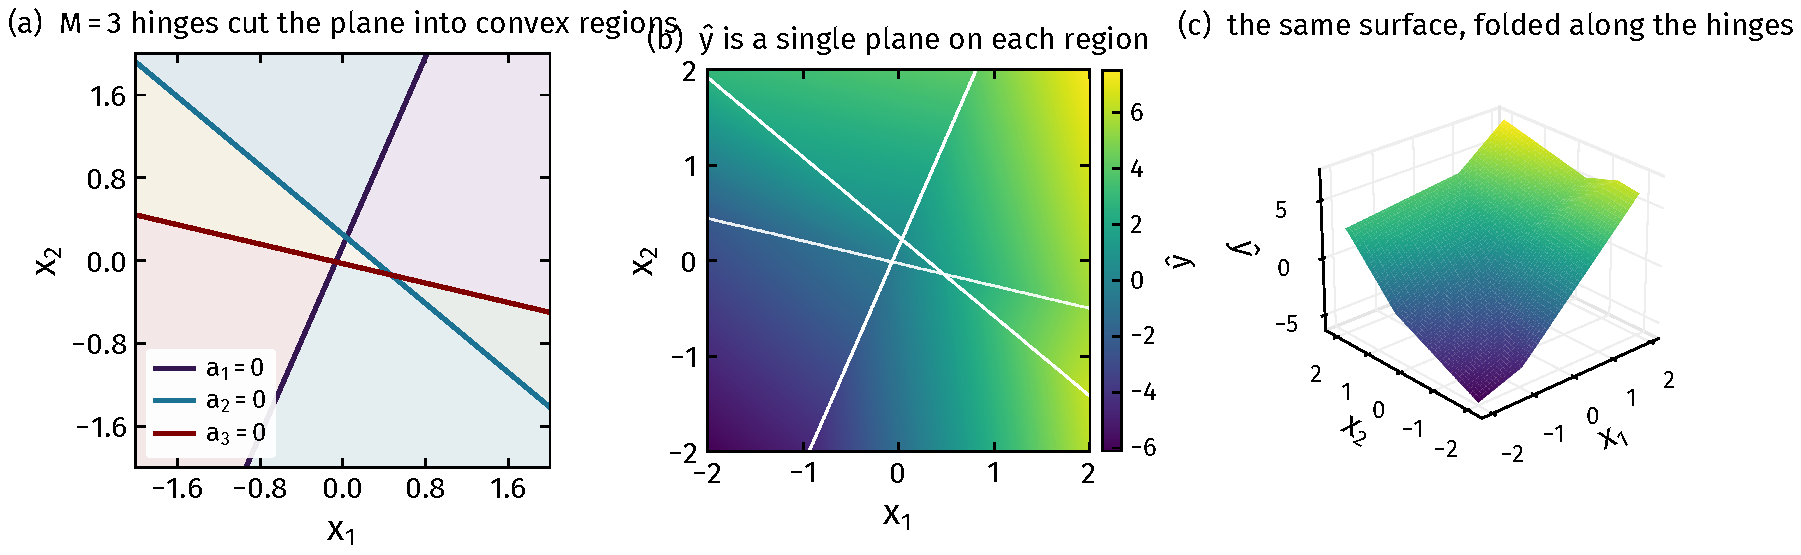
\includegraphics[height=0.50\textheight]{buildup2d}
  \end{center}
  \figcap[0.95]{(a) the three lines $a_j=0$ cut the plane into
  \alert{convex regions}, one per activation pattern.
  (b) $\hat y$ is a single plane on each region, with the borders in
  white. (c) the same output as a landscape --- one surface, folded
  along the hinge lines.}
\end{frame}

\begin{frame}{The general case}
  \begin{columns}[T, onlytextwidth]
    \begin{column}{0.45\textwidth}
      \centering
      \begin{tikzpicture}[>=Stealth, line width=0.7pt,
      scale=0.54, transform shape, font=\normalsize]
    \foreach \i/\y in {1/2.3, 2/0.0, 3/-2.3}
      \plainunit{i\i}{(0,\y)}{black!55}{$x_{\i}$};
    \foreach \i/\y in {1/2.3, 2/0.0, 3/-2.3}
      \unit{h\i}{(3.0,\y)}{shc}{$z_{\i}$};
    \foreach \i/\y in {1/1.2, 2/-1.2}
      \plainunit{o\i}{(6.0,\y)}{dpc}{$\hat y_{\i}$};
    \foreach \i in {1,2,3} \foreach \j in {1,2,3}
      \draw[->, black!25] (i\i)--(h\j);
    \foreach \i in {1,2,3} \foreach \j in {1,2}
      \draw[->, black!35] (h\i)--(o\j);
  \end{tikzpicture}
      \\[0.1em]
      \figsource{$D=3$ inputs, $M=3$ hidden units, $K=2$ outputs
      --- $3(3{+}1)+2(3{+}1)=20$ parameters.}
    \end{column}
    \hfill
    \begin{column}{0.51\textwidth}
      \vspace{0.3em}
      {\small $D$ inputs, $M$ hidden units, $K$ outputs:}
      \[
        z_j = h\Big(\textstyle\sum_{i=1}^{D} w^{(1)}_{ji}x_i
        + w^{(1)}_{j0}\Big)
        \tag{B\&B 6.1--6.2}
      \]
      \[
        \hat y_k = \textstyle\sum_{j=1}^{M} w^{(2)}_{kj}z_j
        + w^{(2)}_{k0}
        \tag{B\&B 6.3}
      \]
      \vspace{-0.4em}
      {\small
      \begin{itemize}\setlength{\itemsep}{2pt}
        \item In matrix form:
              $\hat{\mathbf{y}}
              =\mathbf{W}^{(2)}h\big(\mathbf{W}^{(1)}\mathbf{x}\big)$
              with biases absorbed as $x_0\!=\!1$, $z_0\!=\!1$
      \end{itemize}}
    \end{column}
  \end{columns}
\end{frame}

\begin{frame}{Terminology}
  \begin{columns}[T, onlytextwidth]
    \begin{column}{0.52\textwidth}
      \centering
      \begin{tikzpicture}[>=Stealth, line width=0.7pt,
      scale=0.54, transform shape, font=\normalsize]
    \foreach \i/\y in {1/1.4, 2/-1.4}
      \plainunit{i\i}{(0,\y)}{black!55}{};
    \foreach \i/\y in {1/2.4, 2/0.0, 3/-2.4}
      \unit{h\i}{(3.2,\y)}{shc}{};
    \plainunit{o}{(6.4,0)}{dpc}{};
    \foreach \i in {1,2} \foreach \j in {1,2,3}
      \draw[->, black!25] (i\i)--(h\j);
    \foreach \i in {1,2,3} \draw[->, black!35] (h\i)--(o);
    \node[font=\small] at (0,3.4) {input layer};
    \node[font=\small, shc] at (3.2,4.1) {hidden layer};
    \node[font=\small, dpc] at (6.4,3.4) {output layer};
    \node[font=\small, black!70] at (1.6,-3.7) {$\mathbf{W}^{(1)}$};
    \node[font=\small, black!70] at (4.8,-3.7) {$\mathbf{W}^{(2)}$};
    \draw[decorate, decoration={brace, amplitude=5pt, mirror}, black!45]
      (-0.7,-3.1) -- (7.1,-3.1);
    \node[font=\small, black!70] at (3.2,-4.6)
      {feed-forward, fully connected};
  \end{tikzpicture}
      \\[0.1em]
      \figsource{The standard vocabulary for the parts of a network.}
    \end{column}
    \hfill
    \begin{column}{0.44\textwidth}
      \vspace{0.3em}
      {\small
      \begin{itemize}\setlength{\itemsep}{2pt}
        \item \alert{input} / \alert{hidden} / \alert{output layer}
        \item weights (slopes) and \alert{biases} (offsets)
        \item pre-activations $a_j$, activations $z_j$
        \item \alert{fully connected, feed-forward}; one hidden
              layer $=$ \alert{shallow}
        \item with one or more hidden layers, also called a
              \alert{multi-layer perceptron}
      \end{itemize}}
    \end{column}
  \end{columns}
\end{frame}

\begin{frame}{How many regions?}
  \begin{center}
    
\includegraphics[height=0.425\textheight]{regions}
  \end{center}
  \figcap[0.95]{(a) the bound against the number of units, for several
  input dimensions $D$ (log--log). (b) three networks of different
  width on a scalar input; markers are the joints.}
  \vspace{0.1em}
  {\footnotesize
  \begin{itemize}\setlength{\itemsep}{1pt}
    \item \alert{Zaslavsky (1975):} $M$ hyperplanes in general
          position in $\mathbb{R}^{D}$ create at most
          $\sum_{j=0}^{D}\binom{M}{j}$ regions
    \item $D=10$, $M=100$ units ($\approx 1200$ parameters) already
          exceeds $10^{13}$ regions
  \end{itemize}}
\end{frame}

\begin{frame}{Other activation functions}
  \begin{center}
    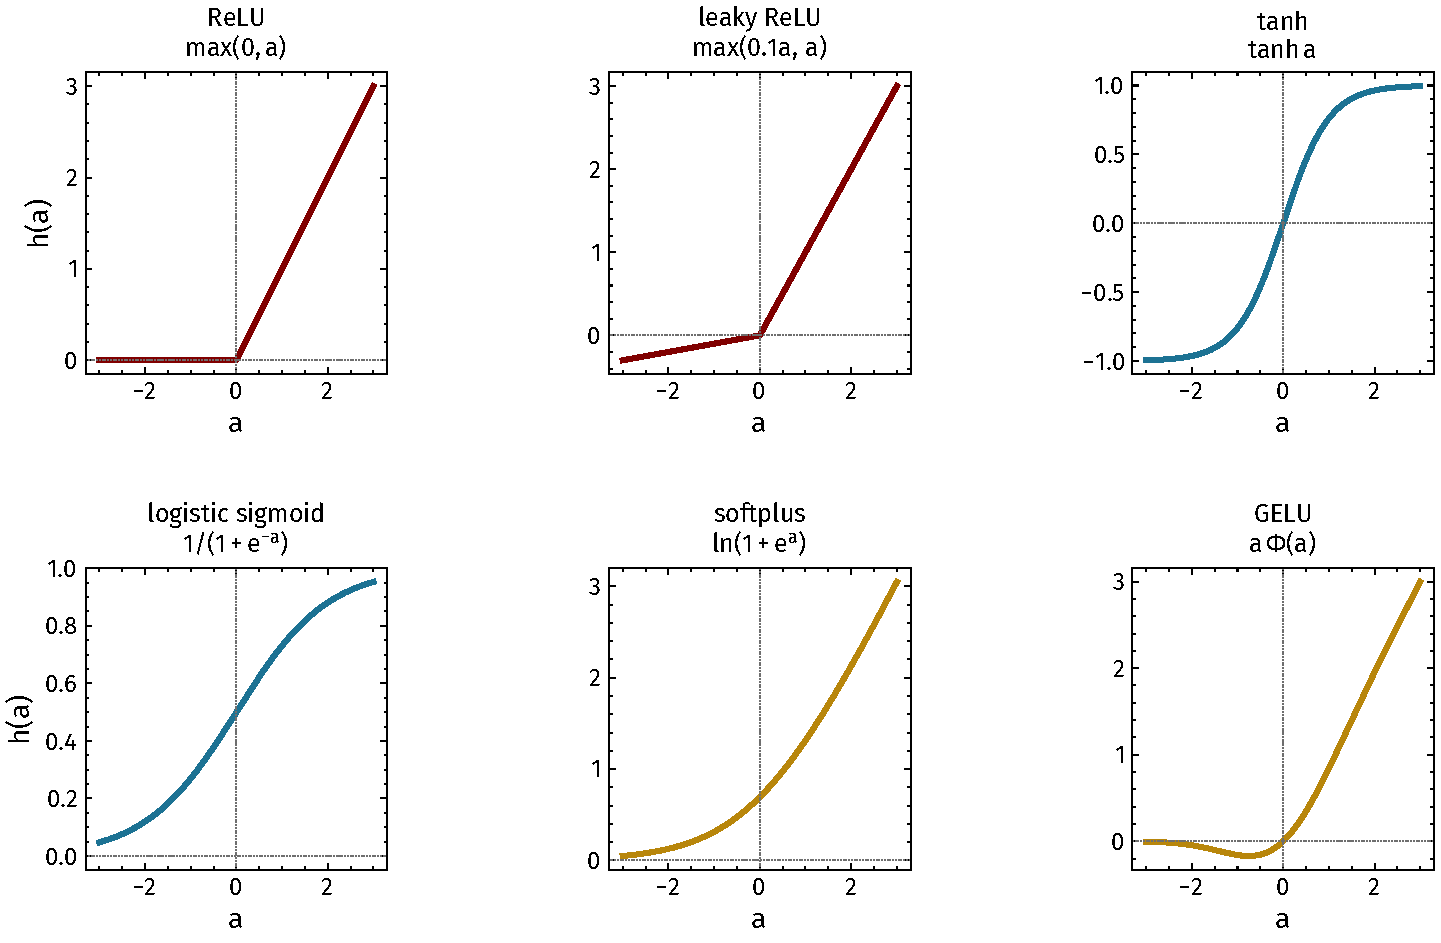
\includegraphics[height=0.60\textheight]{activations}
  \end{center}
  \figcap[0.92]{ReLU is the modern default; $\tanh$ and the logistic
  sigmoid were historically standard; softplus and GELU are smooth
  relatives of ReLU. Only the \emph{shape} changes --- the
  architecture does not.}
\end{frame}

% =====================================================================
\section{Universal Approximation}
% =====================================================================

\begin{frame}{The question}
  With enough hidden units, how much can one hidden layer express?
  \vspace{0.5em}
  \begin{itemize}\setlength{\itemsep}{3pt}
    \item Every function the network computes is \alert{continuous
          and piecewise linear} (with ReLU)
    \item Adding a unit adds a joint --- one more piece to play with
    \item So the question is whether piecewise-linear functions can
          get \alert{arbitrarily close} to an arbitrary continuous
          target
  \end{itemize}
  \vspace{0.5em}
  \begin{redhighlight}
    The answer is yes, and for $D=1$ with ReLU we can prove it
    \alert{constructively} --- the proof tells us exactly which
    weights to use.
  \end{redhighlight}
\end{frame}

\begin{frame}{Universal approximation: the statement}
  \begin{theorem}[Universal approximation; Cybenko 1989, Hornik 1991]
    Let $h:\mathbb{R}\to\mathbb{R}$ be continuous and
    \alert{not a polynomial}, let $\mathcal{K}\subset\mathbb{R}^{D}$
    be compact, and let $f:\mathcal{K}\to\mathbb{R}$ be continuous.
    Then for every $\varepsilon>0$ there exist a finite $M$ and
    weights $\mathbf{w}^{(1)}_j\in\mathbb{R}^{D}$,
    $w^{(1)}_{j0},w^{(2)}_j\in\mathbb{R}$ such that
    \[
      \hat y(\mathbf{x})
      = w^{(2)}_0+\sum_{j=1}^{M}w^{(2)}_j\,
        h\big(\mathbf{w}^{(1)\top}_j\mathbf{x}+w^{(1)}_{j0}\big)
      \quad\text{satisfies}\quad
      \sup_{\mathbf{x}\in\mathcal{K}}\big|f(\mathbf{x})
      -\hat y(\mathbf{x})\big| < \varepsilon .
    \]
  \end{theorem}
  \vspace{0.1em}
  {\footnotesize
  \begin{itemize}\setlength{\itemsep}{0pt}
    \item One hidden layer is enough --- \alert{width}, not depth,
          is the resource being spent
    \item ``Not a polynomial'' is \alert{necessary}: if
          $\deg h = p$, every network output is a polynomial of
          degree $\le p$, and those are not dense in
          $C(\mathcal{K})$ \hfill{\scriptsize (Leshno et al., 1993)}
  \end{itemize}}
\end{frame}

\begin{frame}{Lemma 1: two ReLUs make a ramp}
  \begin{lemmax}[Ramps and steps]
    For $a\in\mathbb{R}$ and $\delta>0$ define
    $g_{\delta}(x)=\frac{1}{\delta}\big[h(x-a)-h(x-a-\delta)\big]$
    with $h=\mathrm{ReLU}$. Then $g_{\delta}$ is continuous,
    $g_{\delta}\equiv 0$ for $x\le a$, $g_{\delta}\equiv 1$ for
    $x\ge a+\delta$, and it is linear in between. Hence
    $g_{\delta}(x)\to\mathbb{1}[x>a]$ pointwise as
    $\delta\downarrow 0$.
  \end{lemmax}
  \vspace{0.2em}
  {\footnotesize
  \emph{Proof.} Check the three cases directly.
  For $x\le a$ both ReLUs vanish. For $a<x<a+\delta$ the first is
  $x-a$ and the second still vanishes, giving $(x-a)/\delta$. For
  $x\ge a+\delta$ the difference is
  $(x-a)-(x-a-\delta)=\delta$, so $g_{\delta}=1$. \hfill$\square$}
  \vspace{0.4em}
  \begin{redhighlight}
    {\small Two hidden units buy a \alert{switch}. Everything else is
    bookkeeping: a sum of switches is a staircase, and a staircase
    with fine enough steps tracks any continuous function.}
  \end{redhighlight}
\end{frame}

\begin{frame}{Lemma 2: the interpolant \emph{is} a network}
  \begin{lemmax}[Exact representation of a piecewise-linear function]
    {\small Let $x_0<x_1<\dots<x_M$ and let $\hat y$ be the continuous
    function that is linear on each $[x_{j-1},x_j]$ with slope
    $s_j$. Then for all $x\in[x_0,x_M]$
    \[
      \hat y(x) \;=\; \hat y(x_0) + s_1\,h(x-x_0)
      + \sum_{j=1}^{M-1}\big(s_{j+1}-s_j\big)\,h(x-x_j),
    \]
    a shallow ReLU network with $M$ hidden units whose output weights
    are the \alert{slope increments}.}
  \end{lemmax}
  \vspace{0.1em}
  {\scriptsize
  \emph{Proof.} Both sides are continuous and piecewise linear with the
  same breakpoints, so it suffices to match value and slope. At $x=x_0$
  every $h(\cdot)$ term vanishes, so both sides equal $\hat y(x_0)$. On
  $(x_{k-1},x_k)$ the active terms are those with $x_j<x$, so the
  right-hand slope telescopes to
  $s_1+\sum_{j=1}^{k-1}(s_{j+1}-s_j)=s_k$. \hfill$\square$}
\end{frame}

\begin{frame}{Proof of the theorem for $D=1$, ReLU}
  \vspace{0.15em}
  {\footnotesize
  Let $f$ be continuous on $[0,1]$ and fix $\varepsilon>0$.}
  \begin{itemize}\setlength{\itemsep}{3pt}
    \item \focus{1}{\textbf{Step 1 (uniform continuity).} $[0,1]$ is
          compact, so $f$ is uniformly continuous: there is
          $\delta>0$ with $|f(u)-f(v)|<\varepsilon/2$ whenever
          $|u-v|<\delta$.}
    \item \focus{2}{\textbf{Step 2 (choose the grid).} Take
          $M=\lceil 1/\delta\rceil$ and $x_j=j/M$, so the mesh
          $1/M<\delta$. Let $\hat y$ be the piecewise-linear
          interpolant of $f$ at these knots.}
    \item \focus{3}{\textbf{Step 3 (bound the error).} For
          $x\in[x_{j-1},x_j]$, $\hat y(x)$ is a convex combination
          $\lambda f(x_{j-1})+(1-\lambda)f(x_j)$, so
          $|\hat y(x)-f(x_{j-1})|\le\max\{|f(x_{j-1})-f(x_j)|,0\}
          <\varepsilon/2$, giving
          $|f(x)-\hat y(x)|\le|f(x)-f(x_{j-1})|
          +|f(x_{j-1})-\hat y(x)|<\varepsilon$.}
    \item \focus{4}{\textbf{Step 4 (it is a network).} By Lemma~2,
          $\hat y$ is exactly a shallow ReLU network with $M$ hidden
          units. Therefore
          $\sup_{x\in[0,1]}|f(x)-\hat y(x)|<\varepsilon$.
          \hfill$\square$}
  \end{itemize}
\end{frame}

\begin{frame}{The construction, drawn}
  \begin{center}
    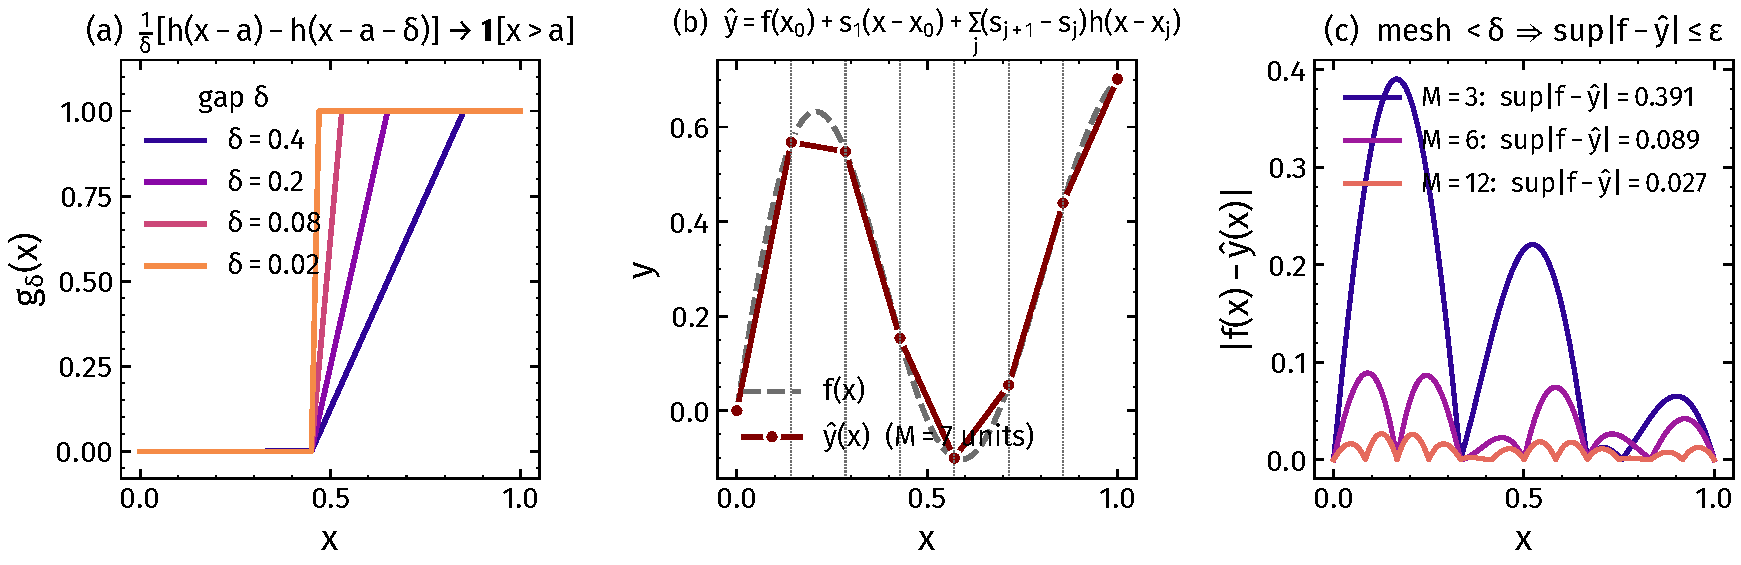
\includegraphics[height=0.485\textheight]{ua_construction}
  \end{center}
  \figcap[0.95]{(a) Lemma~1: as the gap $\delta$ shrinks, the scaled
  ReLU difference becomes a unit step. (b) Lemma~2: the interpolant
  through the knots $x_j$ is written exactly as a sum of ReLUs whose
  output weights are the slope increments. (c) Step~3: refining the
  mesh drives $\sup|f-\hat y|$ down.}
\end{frame}

\begin{frame}{Using the theorem: how fast does the error fall?}
  \begin{columns}[T, onlytextwidth]
    \begin{column}{0.50\textwidth}
      \centering
      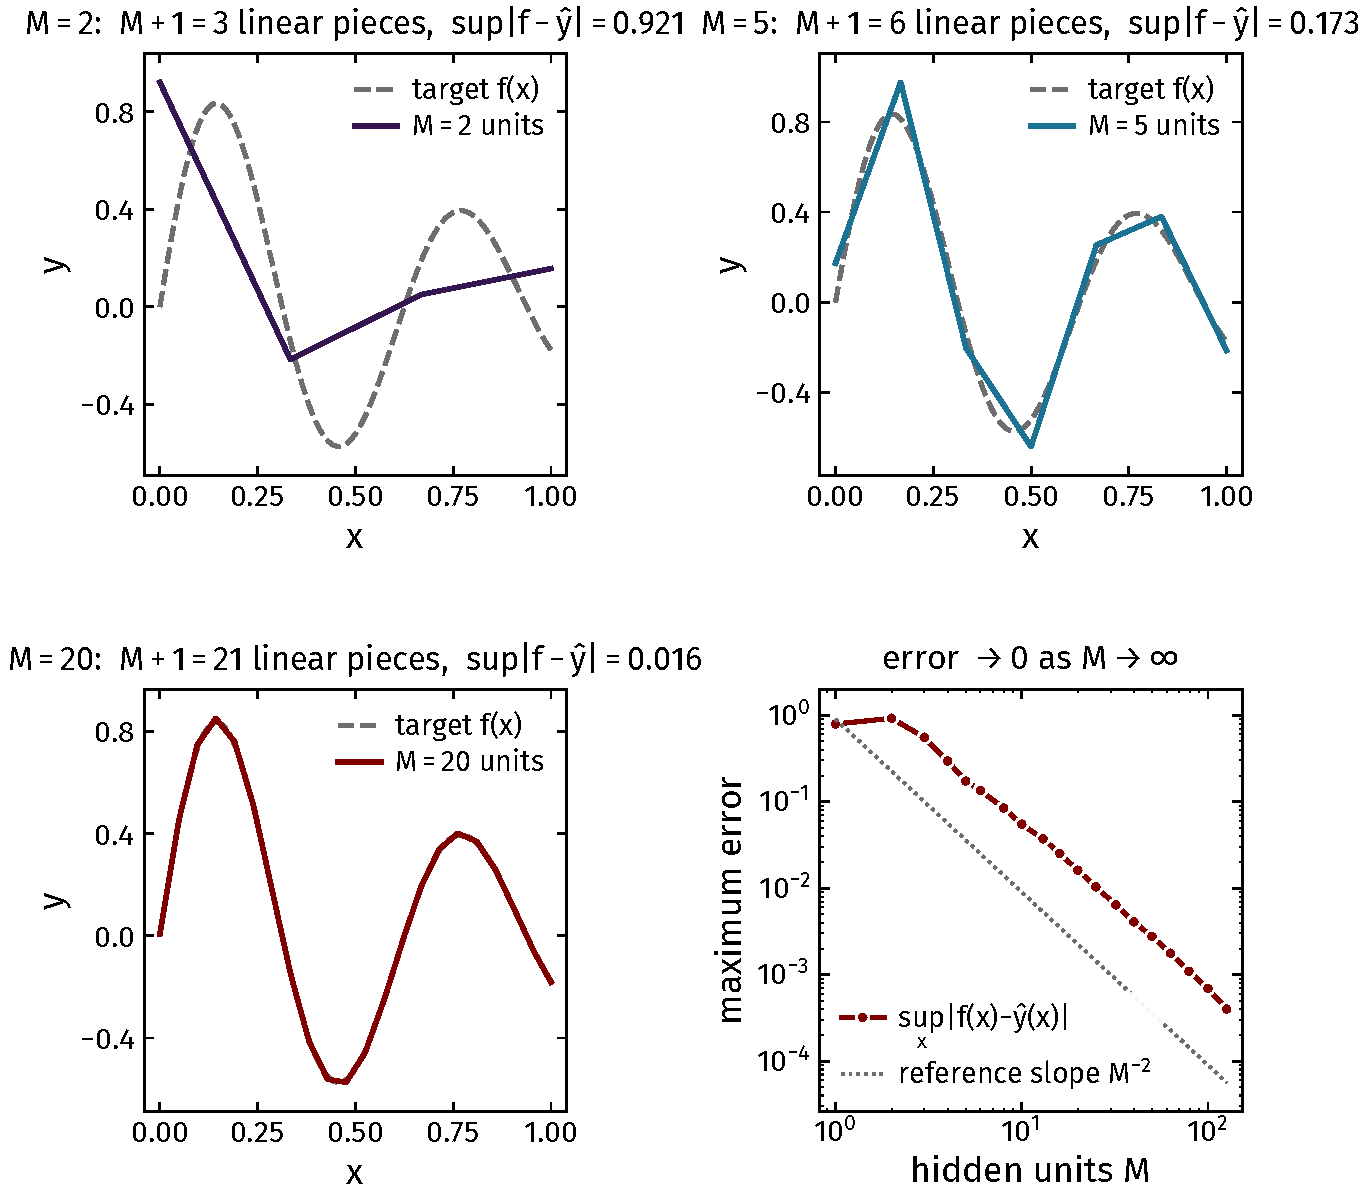
\includegraphics[height=0.74\textheight]{approximate}
    \end{column}
    \hfill
    \begin{column}{0.46\textwidth}
      \vspace{0.4em}
      {\small
      If $f$ is Lipschitz with constant $L$ on $[0,1]$, Step~1 lets
      us take $\delta=\varepsilon/(2L)$, so}
      \[
        M \;=\; \big\lceil 2L/\varepsilon \big\rceil
      \]
      {\small
      units suffice --- \alert{linear} in $L/\varepsilon$. If $f$ is
      also $C^2$, interpolation theory sharpens this to
      $\sup|f-\hat y|\le \tfrac18\lVert f''\rVert_\infty M^{-2}$.}
      \vspace{0.3em}
      {\small
      \begin{itemize}\setlength{\itemsep}{2pt}
        \item Panels: $M=2$, $5$, $20$ units on one target
        \item Last panel: the measured $\sup$ error, tracking the
              predicted $M^{-2}$ slope
      \end{itemize}}
    \end{column}
  \end{columns}
\end{frame}

\begin{frame}{What the theorem does \emph{not} say}
  \begin{itemize}\setlength{\itemsep}{4pt}
    \item \alert{It is an existence result.} It says good weights
          exist; it does not say gradient descent will find them,
          nor that they are learnable from finite data.
    \item \alert{It says nothing about generalisation.} Fitting a
          training set arbitrarily well is not the goal --- recall
          the irreducible noise term.
    \item \alert{The width can be astronomical.} Repeating the grid
          argument in $D$ dimensions needs
          $M=O\big((L/\varepsilon)^{D}\big)$ units: the
          \alert{curse of dimensionality}.
  \end{itemize}
  \vspace{0.4em}
  \begin{redhighlight}
    This last point is the opening argument of Class~7: \alert{depth}
    buys regions exponentially in the number of layers, where width
    buys them only polynomially.
  \end{redhighlight}
\end{frame}

% =====================================================================
\section{Training}
% =====================================================================

\begin{frame}{Same error, harder landscape}
  Sum-of-squares error, now with a network inside
  (Bishop \& Bishop, 2024, \S6.1):
  \[
    E(\mathbf{w}) = \tfrac{1}{2}\sum_{n=1}^{N}
    \big\lVert \hat{\mathbf{y}}(\mathbf{x}_n,\mathbf{w})
    - \mathbf{y}_n\big\rVert^2
  \]
  \vspace{-0.3em}
  \begin{itemize}\setlength{\itemsep}{1pt}
    \item {\small Parameters sit \emph{inside} $h(\cdot)$, so
          $\nabla E=\mathbf{0}$ has \alert{no closed form} ---
          the normal-equations theorem no longer applies}
    \item {\small The error surface is \alert{non-convex}, unlike
          every model so far}
    \item {\small Training: gradient descent and backpropagation
          --- Classes 11--13}
  \end{itemize}
  \mlparallel{normal equations: jump straight to the minimum}
             {gradient descent: walk downhill, non-convex}
\end{frame}

\begin{frame}{Why the surface cannot be convex}
  \begin{propx}[Weight-space symmetries; B\&B \S6.1.1]
    For a network with $M$ hidden units and an odd activation
    ($h(-a)=-h(a)$, e.g.\ $\tanh$), every weight vector
    $\mathbf{w}$ has at least $M!\,2^{M}$ distinct counterparts
    computing the \alert{identical} function.
  \end{propx}
  \vspace{0.1em}
  {\footnotesize
  \emph{Proof.}
  \emph{(i) Sign flip.} Replace
  $\mathbf{w}^{(1)}_j\!\to\!-\mathbf{w}^{(1)}_j$ and
  $w^{(2)}_{kj}\!\to\!-w^{(2)}_{kj}$. Then
  $w^{(2)}_{kj}h(a_j)$ is unchanged since $h$ is odd. There are
  $2^{M}$ such choices.
  \emph{(ii) Permutation.} Relabelling the hidden units permutes
  rows of $\mathbf{W}^{(1)}$ and columns of $\mathbf{W}^{(2)}$
  together, leaving the sum unchanged: $M!$ choices. The two act
  independently. \hfill$\square$}
  \vspace{0.3em}
  \begin{redhighlight}
    {\small Every minimum is repeated at least $M!\,2^{M}$ times.
    A function with many separated global minima cannot be convex
    --- the non-convexity is \alert{structural}, not accidental.}
  \end{redhighlight}
\end{frame}

\begin{frame}{It works: shallow networks fit real data}
  \begin{center}
    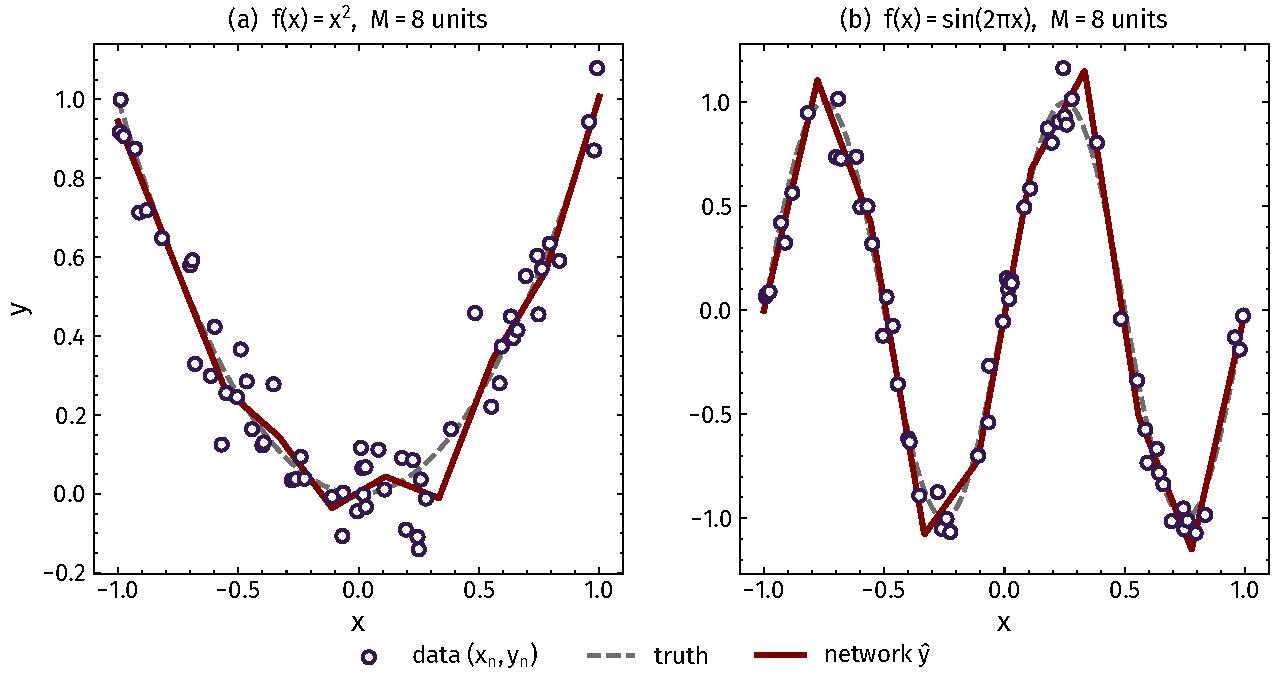
\includegraphics[height=0.525\textheight]{fits}
  \end{center}
  \figcap[0.92]{A shallow ReLU network with $M=8$ units fitted by
  least squares to noisy samples of two functions. The learned units
  place their joints where the data bends; the fit tracks the truth
  without chasing every noisy point.}
\end{frame}

\begin{frame}{The dictionary}
  \centering
  \renewcommand{\arraystretch}{1.12}
  {\footnotesize
  \begin{tabular}{p{0.20\textwidth} p{0.35\textwidth}
                  p{0.35\textwidth}}
    & \textbf{\color{mlc}Linear/Basis-Function Model}
    & \textbf{\color{nnc}Shallow Neural Network}\\
    \hline
    Function class
      & lines, polynomials, RBFs
      & piecewise-linear surfaces\\
    Features
      & $\phi_j(\mathbf{x})$, fixed
      & $z_j=h(a_j)$, learned\\
    Prediction
      & $\mathbf{w}^{\!\top}\boldsymbol{\phi}(\mathbf{x})$
      & $\sum_j w^{(2)}_{kj} z_j + w^{(2)}_{k0}$\\
    Error (regression)
      & sum of squares
      & sum of squares\\
    Optimisation
      & normal equations, convex
      & gradient descent, non-convex\\
    Capacity
      & number of basis functions $M$
      & hidden units $M$, regions
        $\le\sum_{j\le D}\binom{M}{j}$\\
    \hline
  \end{tabular}}
  \vspace{0.5em}
  \begin{redhighlight}
    A shallow network is regression whose basis functions carry
    parameters and are learned from data.
  \end{redhighlight}
\end{frame}

\begin{frame}{Takeaways}
  \vspace{0.1em}
  {\footnotesize
  \begin{enumerate}\setlength{\itemsep}{1pt}
    \item A shallow network puts parameters inside the basis
          functions; the output layer is a \alert{linear regression
          on learned features}
    \item Least squares has a \alert{closed form} and a clean
          geometry --- an orthogonal projection --- only while the
          model is linear in $\mathbf{w}$
    \item With ReLU the family is \alert{piecewise linear}: one
          joint per unit, regions counted by binomial coefficients
    \item \alert{Universal approximation} holds, and for $D=1$ we
          proved it constructively --- but it is existence, and the
          width needed grows like $(L/\varepsilon)^{D}$
    \item The price: \alert{no closed form}, a structurally
          non-convex error surface, gradient-based training
  \end{enumerate}}
  \vspace{0.1em}
  \begin{redhighlight}
    {\footnotesize Class~6: the same architecture for
    \alert{classification} --- sigmoid/softmax outputs and
    cross-entropy error.}
  \end{redhighlight}
\end{frame}

\begin{frame}{References}
  \footnotesize
  \begin{itemize}\setlength{\itemsep}{3pt}
    \item C.~M.~Bishop \& H.~Bishop. \textit{Deep Learning:
          Foundations and Concepts.} Springer, 2024.
          \S4.1 (basis functions, least squares, the geometry of
          the normal equations), \S4.2 (decision theory for
          regression), \S6.1 (feed-forward networks, weight-space
          symmetries). Figure~4.3 reproduced as printed.
    \item S.~J.~D.~Prince. \textit{Understanding Deep Learning.}
          MIT Press, 2023. Ch.~3 --- shallow networks, the
          piecewise-linear picture, region counting.
    \item G.~Cybenko, \textit{Math.\ Control Signals Systems}, 1989;
          K.~Hornik, \textit{Neural Networks}, 1991;
          M.~Leshno et al., \textit{Neural Networks}, 1993
          (non-polynomial activations).
    \item T.~Zaslavsky, \textit{Facing up to Arrangements}, AMS,
          1975 --- the region count.

  \end{itemize}
\end{frame}

\begin{frame}[standout]
  Questions?
\end{frame}

\end{document}
